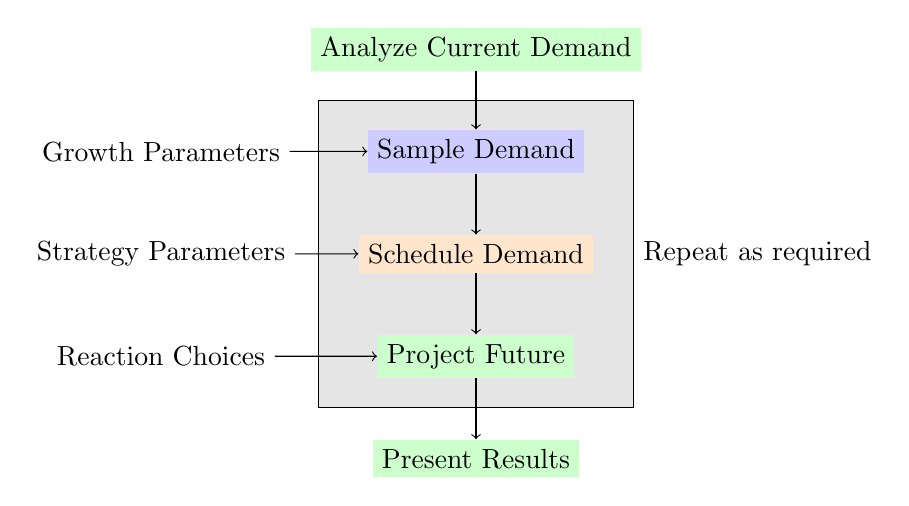
\begin{tikzpicture}[xscale=2,yscale=1.3]
  \draw[fill=black!10] (0,1.5) rectangle (2,4.5);
  \node[right] at (2,3) {Repeat as required};
  \node[fill=green!20] (analyse) at (1,5) {Analyze Current Demand};
  \node[fill=blue!20] (sample) at (1,4) {Sample Demand};
  \node (increase) at (-1,4) {Growth Parameters};
  \node (params) at (-1,3) {Strategy Parameters};
  \node (reaction) at (-1,2) {Reaction Choices};
  \node[fill=orange!20] (schedule) at (1,3) {Schedule Demand};
  \node[fill=green!20] (project) at (1,2) {Project Future};
  \node[fill=green!20] (present) at (1,1) {Present Results};
  \draw[->] (analyse) -- (sample);
  \draw[->] (increase) -- (sample);
  \draw[->] (sample) -- (schedule);
  \draw[->] (params) -- (schedule);
  \draw[->] (schedule) -- (project);
  \draw[->] (reaction) -- (project);
  \draw[->] (project) -- (present);
\end{tikzpicture}
